\usetikzlibrary{arrows.meta,calc}
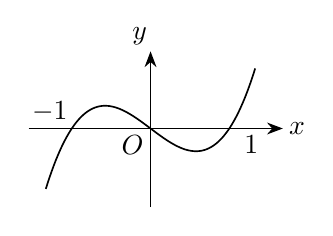
\begin{tikzpicture}[x=1cm,y=1cm,line width=.6pt,>=Stealth]
\draw[->] (-1.55,0)--(1.68,0) node[anchor=west,inner sep=0pt,xshift=2pt] {$x$};
\draw[->] (0,-1.0)--(0,0.98) node[anchor=south east,inner sep=0pt,yshift=2pt,xshift=-1pt] {$y$};
\draw[domain=-1.33:1.33,samples=161] plot (\x,{0.75*(\x*\x*\x-\x)});
\node[anchor=north east,inner sep=0pt] at (-0.08,-0.08) {$O$};
\node[anchor=south,inner sep=0pt] at (-1.28,0.08) {$-1$};
\node[anchor=north,inner sep=0pt] at (1.28,-0.08) {$1$};
\end{tikzpicture}
